% Created by tikzDevice version 0.12.3 on 2020-05-27 23:04:56
% !TEX encoding = UTF-8 Unicode
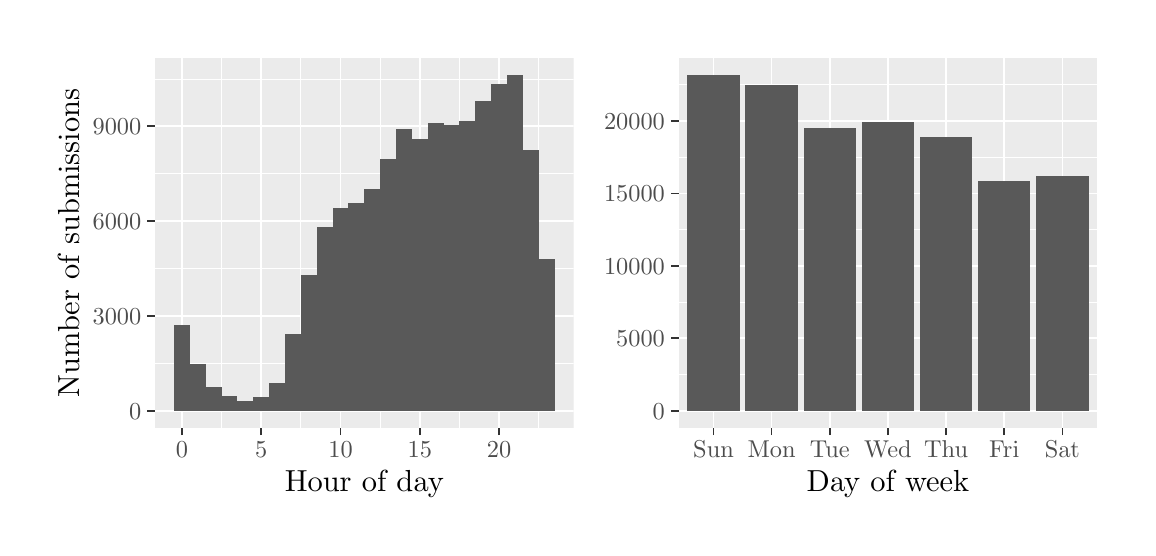
\begin{tikzpicture}[x=1pt,y=1pt]
\definecolor{fillColor}{RGB}{255,255,255}
\path[use as bounding box,fill=fillColor,fill opacity=0.00] (0,0) rectangle (397.48,180.67);
\begin{scope}
\path[clip] (  0.00,  0.00) rectangle (397.48,180.67);
\definecolor{drawColor}{RGB}{255,255,255}
\definecolor{fillColor}{RGB}{255,255,255}

\path[draw=drawColor,line width= 0.6pt,line join=round,line cap=round,fill=fillColor] (  0.00,  0.00) rectangle (397.48,180.68);
\end{scope}
\begin{scope}
\path[clip] (  5.50,  5.50) rectangle (202.78,175.17);
\definecolor{drawColor}{RGB}{255,255,255}
\definecolor{fillColor}{RGB}{255,255,255}

\path[draw=drawColor,line width= 0.6pt,line join=round,line cap=round,fill=fillColor] (  5.50,  5.50) rectangle (202.78,175.17);
\end{scope}
\begin{scope}
\path[clip] ( 46.01, 36.19) rectangle (197.28,169.67);
\definecolor{fillColor}{gray}{0.92}

\path[fill=fillColor] ( 46.01, 36.19) rectangle (197.28,169.67);
\definecolor{drawColor}{RGB}{255,255,255}

\path[draw=drawColor,line width= 0.3pt,line join=round] ( 46.01, 59.38) --
	(197.28, 59.38);

\path[draw=drawColor,line width= 0.3pt,line join=round] ( 46.01, 93.64) --
	(197.28, 93.64);

\path[draw=drawColor,line width= 0.3pt,line join=round] ( 46.01,127.89) --
	(197.28,127.89);

\path[draw=drawColor,line width= 0.3pt,line join=round] ( 46.01,162.15) --
	(197.28,162.15);

\path[draw=drawColor,line width= 0.3pt,line join=round] ( 70.08, 36.19) --
	( 70.08,169.67);

\path[draw=drawColor,line width= 0.3pt,line join=round] ( 98.72, 36.19) --
	( 98.72,169.67);

\path[draw=drawColor,line width= 0.3pt,line join=round] (127.37, 36.19) --
	(127.37,169.67);

\path[draw=drawColor,line width= 0.3pt,line join=round] (156.02, 36.19) --
	(156.02,169.67);

\path[draw=drawColor,line width= 0.3pt,line join=round] (184.67, 36.19) --
	(184.67,169.67);

\path[draw=drawColor,line width= 0.6pt,line join=round] ( 46.01, 42.25) --
	(197.28, 42.25);

\path[draw=drawColor,line width= 0.6pt,line join=round] ( 46.01, 76.51) --
	(197.28, 76.51);

\path[draw=drawColor,line width= 0.6pt,line join=round] ( 46.01,110.76) --
	(197.28,110.76);

\path[draw=drawColor,line width= 0.6pt,line join=round] ( 46.01,145.02) --
	(197.28,145.02);

\path[draw=drawColor,line width= 0.6pt,line join=round] ( 55.75, 36.19) --
	( 55.75,169.67);

\path[draw=drawColor,line width= 0.6pt,line join=round] ( 84.40, 36.19) --
	( 84.40,169.67);

\path[draw=drawColor,line width= 0.6pt,line join=round] (113.05, 36.19) --
	(113.05,169.67);

\path[draw=drawColor,line width= 0.6pt,line join=round] (141.70, 36.19) --
	(141.70,169.67);

\path[draw=drawColor,line width= 0.6pt,line join=round] (170.35, 36.19) --
	(170.35,169.67);
\definecolor{fillColor}{gray}{0.35}

\path[fill=fillColor] ( 52.89, 42.25) rectangle ( 58.62, 73.19);

\path[fill=fillColor] ( 58.62, 42.25) rectangle ( 64.35, 59.03);

\path[fill=fillColor] ( 64.35, 42.25) rectangle ( 70.08, 50.93);

\path[fill=fillColor] ( 70.08, 42.25) rectangle ( 75.80, 47.59);

\path[fill=fillColor] ( 75.80, 42.25) rectangle ( 81.53, 45.76);

\path[fill=fillColor] ( 81.53, 42.25) rectangle ( 87.26, 47.30);

\path[fill=fillColor] ( 87.26, 42.25) rectangle ( 92.99, 52.11);

\path[fill=fillColor] ( 92.99, 42.25) rectangle ( 98.72, 70.07);

\path[fill=fillColor] ( 98.72, 42.25) rectangle (104.45, 91.31);

\path[fill=fillColor] (104.45, 42.25) rectangle (110.18,108.51);

\path[fill=fillColor] (110.18, 42.25) rectangle (115.91,115.68);

\path[fill=fillColor] (115.91, 42.25) rectangle (121.64,117.28);

\path[fill=fillColor] (121.64, 42.25) rectangle (127.37,122.31);

\path[fill=fillColor] (127.37, 42.25) rectangle (133.10,133.33);

\path[fill=fillColor] (133.10, 42.25) rectangle (138.83,143.92);

\path[fill=fillColor] (138.83, 42.25) rectangle (144.56,140.54);

\path[fill=fillColor] (144.56, 42.25) rectangle (150.29,146.15);

\path[fill=fillColor] (150.29, 42.25) rectangle (156.02,145.34);

\path[fill=fillColor] (156.02, 42.25) rectangle (161.75,146.89);

\path[fill=fillColor] (161.75, 42.25) rectangle (167.48,154.13);

\path[fill=fillColor] (167.48, 42.25) rectangle (173.21,160.31);

\path[fill=fillColor] (173.21, 42.25) rectangle (178.94,163.61);

\path[fill=fillColor] (178.94, 42.25) rectangle (184.67,136.52);

\path[fill=fillColor] (184.67, 42.25) rectangle (190.40, 96.98);
\end{scope}
\begin{scope}
\path[clip] (  0.00,  0.00) rectangle (397.48,180.67);
\definecolor{drawColor}{gray}{0.30}

\node[text=drawColor,anchor=base east,inner sep=0pt, outer sep=0pt, scale=  0.88] at ( 41.06, 39.22) {0};

\node[text=drawColor,anchor=base east,inner sep=0pt, outer sep=0pt, scale=  0.88] at ( 41.06, 73.48) {3000};

\node[text=drawColor,anchor=base east,inner sep=0pt, outer sep=0pt, scale=  0.88] at ( 41.06,107.73) {6000};

\node[text=drawColor,anchor=base east,inner sep=0pt, outer sep=0pt, scale=  0.88] at ( 41.06,141.99) {9000};
\end{scope}
\begin{scope}
\path[clip] (  0.00,  0.00) rectangle (397.48,180.67);
\definecolor{drawColor}{gray}{0.20}

\path[draw=drawColor,line width= 0.6pt,line join=round] ( 43.26, 42.25) --
	( 46.01, 42.25);

\path[draw=drawColor,line width= 0.6pt,line join=round] ( 43.26, 76.51) --
	( 46.01, 76.51);

\path[draw=drawColor,line width= 0.6pt,line join=round] ( 43.26,110.76) --
	( 46.01,110.76);

\path[draw=drawColor,line width= 0.6pt,line join=round] ( 43.26,145.02) --
	( 46.01,145.02);
\end{scope}
\begin{scope}
\path[clip] (  0.00,  0.00) rectangle (397.48,180.67);
\definecolor{drawColor}{gray}{0.20}

\path[draw=drawColor,line width= 0.6pt,line join=round] ( 55.75, 33.44) --
	( 55.75, 36.19);

\path[draw=drawColor,line width= 0.6pt,line join=round] ( 84.40, 33.44) --
	( 84.40, 36.19);

\path[draw=drawColor,line width= 0.6pt,line join=round] (113.05, 33.44) --
	(113.05, 36.19);

\path[draw=drawColor,line width= 0.6pt,line join=round] (141.70, 33.44) --
	(141.70, 36.19);

\path[draw=drawColor,line width= 0.6pt,line join=round] (170.35, 33.44) --
	(170.35, 36.19);
\end{scope}
\begin{scope}
\path[clip] (  0.00,  0.00) rectangle (397.48,180.67);
\definecolor{drawColor}{gray}{0.30}

\node[text=drawColor,anchor=base,inner sep=0pt, outer sep=0pt, scale=  0.88] at ( 55.75, 25.18) {0};

\node[text=drawColor,anchor=base,inner sep=0pt, outer sep=0pt, scale=  0.88] at ( 84.40, 25.18) {5};

\node[text=drawColor,anchor=base,inner sep=0pt, outer sep=0pt, scale=  0.88] at (113.05, 25.18) {10};

\node[text=drawColor,anchor=base,inner sep=0pt, outer sep=0pt, scale=  0.88] at (141.70, 25.18) {15};

\node[text=drawColor,anchor=base,inner sep=0pt, outer sep=0pt, scale=  0.88] at (170.35, 25.18) {20};
\end{scope}
\begin{scope}
\path[clip] (  0.00,  0.00) rectangle (397.48,180.67);
\definecolor{drawColor}{RGB}{0,0,0}

\node[text=drawColor,anchor=base,inner sep=0pt, outer sep=0pt, scale=  1.10] at (121.64, 13.14) {Hour of day};
\end{scope}
\begin{scope}
\path[clip] (  0.00,  0.00) rectangle (397.48,180.67);
\definecolor{drawColor}{RGB}{0,0,0}

\node[text=drawColor,rotate= 90.00,anchor=base,inner sep=0pt, outer sep=0pt, scale=  1.10] at ( 18.58,102.93) {Number of submissions};
\end{scope}
\begin{scope}
\path[clip] (202.78,  5.50) rectangle (391.98,175.17);
\definecolor{drawColor}{RGB}{255,255,255}
\definecolor{fillColor}{RGB}{255,255,255}

\path[draw=drawColor,line width= 0.6pt,line join=round,line cap=round,fill=fillColor] (202.78,  5.50) rectangle (391.98,175.17);
\end{scope}
\begin{scope}
\path[clip] (235.22, 36.19) rectangle (386.48,169.67);
\definecolor{fillColor}{gray}{0.92}

\path[fill=fillColor] (235.22, 36.19) rectangle (386.48,169.67);
\definecolor{drawColor}{RGB}{255,255,255}

\path[draw=drawColor,line width= 0.3pt,line join=round] (235.22, 55.34) --
	(386.48, 55.34);

\path[draw=drawColor,line width= 0.3pt,line join=round] (235.22, 81.50) --
	(386.48, 81.50);

\path[draw=drawColor,line width= 0.3pt,line join=round] (235.22,107.67) --
	(386.48,107.67);

\path[draw=drawColor,line width= 0.3pt,line join=round] (235.22,133.84) --
	(386.48,133.84);

\path[draw=drawColor,line width= 0.3pt,line join=round] (235.22,160.00) --
	(386.48,160.00);

\path[draw=drawColor,line width= 0.6pt,line join=round] (235.22, 42.25) --
	(386.48, 42.25);

\path[draw=drawColor,line width= 0.6pt,line join=round] (235.22, 68.42) --
	(386.48, 68.42);

\path[draw=drawColor,line width= 0.6pt,line join=round] (235.22, 94.59) --
	(386.48, 94.59);

\path[draw=drawColor,line width= 0.6pt,line join=round] (235.22,120.75) --
	(386.48,120.75);

\path[draw=drawColor,line width= 0.6pt,line join=round] (235.22,146.92) --
	(386.48,146.92);

\path[draw=drawColor,line width= 0.6pt,line join=round] (247.83, 36.19) --
	(247.83,169.67);

\path[draw=drawColor,line width= 0.6pt,line join=round] (268.83, 36.19) --
	(268.83,169.67);

\path[draw=drawColor,line width= 0.6pt,line join=round] (289.84, 36.19) --
	(289.84,169.67);

\path[draw=drawColor,line width= 0.6pt,line join=round] (310.85, 36.19) --
	(310.85,169.67);

\path[draw=drawColor,line width= 0.6pt,line join=round] (331.86, 36.19) --
	(331.86,169.67);

\path[draw=drawColor,line width= 0.6pt,line join=round] (352.87, 36.19) --
	(352.87,169.67);

\path[draw=drawColor,line width= 0.6pt,line join=round] (373.88, 36.19) --
	(373.88,169.67);
\definecolor{fillColor}{gray}{0.35}

\path[fill=fillColor] (238.37, 42.25) rectangle (257.28,163.61);

\path[fill=fillColor] (259.38, 42.25) rectangle (278.29,160.07);

\path[fill=fillColor] (280.39, 42.25) rectangle (299.30,144.51);

\path[fill=fillColor] (301.40, 42.25) rectangle (320.31,146.66);

\path[fill=fillColor] (322.41, 42.25) rectangle (341.32,141.27);

\path[fill=fillColor] (343.42, 42.25) rectangle (362.32,125.13);

\path[fill=fillColor] (364.43, 42.25) rectangle (383.33,127.08);
\end{scope}
\begin{scope}
\path[clip] (  0.00,  0.00) rectangle (397.48,180.67);
\definecolor{drawColor}{gray}{0.30}

\node[text=drawColor,anchor=base east,inner sep=0pt, outer sep=0pt, scale=  0.88] at (230.27, 39.22) {0};

\node[text=drawColor,anchor=base east,inner sep=0pt, outer sep=0pt, scale=  0.88] at (230.27, 65.39) {5000};

\node[text=drawColor,anchor=base east,inner sep=0pt, outer sep=0pt, scale=  0.88] at (230.27, 91.56) {10000};

\node[text=drawColor,anchor=base east,inner sep=0pt, outer sep=0pt, scale=  0.88] at (230.27,117.72) {15000};

\node[text=drawColor,anchor=base east,inner sep=0pt, outer sep=0pt, scale=  0.88] at (230.27,143.89) {20000};
\end{scope}
\begin{scope}
\path[clip] (  0.00,  0.00) rectangle (397.48,180.67);
\definecolor{drawColor}{gray}{0.20}

\path[draw=drawColor,line width= 0.6pt,line join=round] (232.47, 42.25) --
	(235.22, 42.25);

\path[draw=drawColor,line width= 0.6pt,line join=round] (232.47, 68.42) --
	(235.22, 68.42);

\path[draw=drawColor,line width= 0.6pt,line join=round] (232.47, 94.59) --
	(235.22, 94.59);

\path[draw=drawColor,line width= 0.6pt,line join=round] (232.47,120.75) --
	(235.22,120.75);

\path[draw=drawColor,line width= 0.6pt,line join=round] (232.47,146.92) --
	(235.22,146.92);
\end{scope}
\begin{scope}
\path[clip] (  0.00,  0.00) rectangle (397.48,180.67);
\definecolor{drawColor}{gray}{0.20}

\path[draw=drawColor,line width= 0.6pt,line join=round] (247.83, 33.44) --
	(247.83, 36.19);

\path[draw=drawColor,line width= 0.6pt,line join=round] (268.83, 33.44) --
	(268.83, 36.19);

\path[draw=drawColor,line width= 0.6pt,line join=round] (289.84, 33.44) --
	(289.84, 36.19);

\path[draw=drawColor,line width= 0.6pt,line join=round] (310.85, 33.44) --
	(310.85, 36.19);

\path[draw=drawColor,line width= 0.6pt,line join=round] (331.86, 33.44) --
	(331.86, 36.19);

\path[draw=drawColor,line width= 0.6pt,line join=round] (352.87, 33.44) --
	(352.87, 36.19);

\path[draw=drawColor,line width= 0.6pt,line join=round] (373.88, 33.44) --
	(373.88, 36.19);
\end{scope}
\begin{scope}
\path[clip] (  0.00,  0.00) rectangle (397.48,180.67);
\definecolor{drawColor}{gray}{0.30}

\node[text=drawColor,anchor=base,inner sep=0pt, outer sep=0pt, scale=  0.88] at (247.83, 25.18) {Sun};

\node[text=drawColor,anchor=base,inner sep=0pt, outer sep=0pt, scale=  0.88] at (268.83, 25.18) {Mon};

\node[text=drawColor,anchor=base,inner sep=0pt, outer sep=0pt, scale=  0.88] at (289.84, 25.18) {Tue};

\node[text=drawColor,anchor=base,inner sep=0pt, outer sep=0pt, scale=  0.88] at (310.85, 25.18) {Wed};

\node[text=drawColor,anchor=base,inner sep=0pt, outer sep=0pt, scale=  0.88] at (331.86, 25.18) {Thu};

\node[text=drawColor,anchor=base,inner sep=0pt, outer sep=0pt, scale=  0.88] at (352.87, 25.18) {Fri};

\node[text=drawColor,anchor=base,inner sep=0pt, outer sep=0pt, scale=  0.88] at (373.88, 25.18) {Sat};
\end{scope}
\begin{scope}
\path[clip] (  0.00,  0.00) rectangle (397.48,180.67);
\definecolor{drawColor}{RGB}{0,0,0}

\node[text=drawColor,anchor=base,inner sep=0pt, outer sep=0pt, scale=  1.10] at (310.85, 13.14) {Day of week};
\end{scope}
\end{tikzpicture}
